\documentclass[11pt]{beamer}

%my colours

%TODO: update framework to match new settings
%DONE: review Veripos service
%DONE: update coords
%DONE: re-word table

\usetheme{metropolis}
\metroset{everytitleformat = regular,progressbar=foot} %settings
\mode<presentation>
%\usecolortheme{dove} %dove
% albatross, beaver, beetle, crane, default, dolphin, dove, orchid, rose, seagull, seahorse, whale, wolverine
%dont use  fly, lily,
%http://mirror.ox.ac.uk/sites/ctan.org/macros/latex/contrib/beamer/doc/beameruserguide.pdf
\setbeamercolor{title separator}{fg = UniBlue}
\setbeamercolor{frametitle}{fg = deepBlue, bg=aBlue!70}

\usepackage{booktabs}
\usepackage[scale=2]{ccicons}

\usepackage{pgfplots}
\usepgfplotslibrary{dateplot}


%coords are in relation to lower right corner
%\logo{\pgfputat{\pgfxy(0,6}{\pgfbox[right,top]{
\includegraphics[width=2.5cm]{logo.png}}}}

\usepackage{tikz}
\addtobeamertemplate{frametitle}{}{%
\begin{tikzpicture}[remember picture,overlay]
\node[anchor=north east,yshift=2pt] at (current page.north east) {
\includegraphics[height=0.8cm]{pic/logo.png}};
%\node[anchor=north east,yshift=2pt] at (current page.north east) {
\includegraphics[height=0.8cm]{./../logo.png}};
\end{tikzpicture}}

%My std preamble for the docs
%\selectlanguage{british}%
\usepackage[british]{babel}
\usepackage{microtype} %better text
\IfFileExists{lmodern.sty}{\usepackage{lmodern}}{} %type 1 vector font
%
\usepackage{lettrine}
\usepackage{listings} %Add list support
\usepackage{colortbl} %colors in TABLES
%\usepackage{tikz,amsmath, amssymb,bm,color}
\usepackage{nicefrac}
\usepackage{lastpage} %get last page

%COLORS
\usepackage{color}
\definecolor{lightgray}{gray}{0.8} %for colortbl
\definecolor{UniBlue}{RGB}{83,121,170}
\definecolor{deepBlue}{HTML}{000066}
\definecolor{blueBgd}{HTML}{99C8FF}
\definecolor{aBlue}{HTML}{1879F7}

%%%%%%%%%%%%%%%%%%%%%%%%%%%%%%%%%%%%%%%%%%%%%%%%%%%%%%%%%%%%%%%%%%
%FOOTNOTES
%nice look after http://www.dedoimedo.com


%%%%%%%%%%%%%%%%%%%%%%%%%%%%%%%%%%%%%%%%%%%%%%%%%%%%%%%%%%%%%%%%%%%
%TABLE SETTINGS
\usepackage{colortbl} %colors in table
\usepackage{rotating} %rotatins within tables
\usepackage{multirow}
\renewcommand{\arraystretch}{1.2} %add padding/spacing
%\usepackage{adjustbox}%rotating and fitting into page
%

\usepackage{booktabs} % To thicken table lines
%define thickness of table lines
\let\mytoprule\toprule
\renewcommand{\toprule}{\mytoprule[0.20em]}
\let\mytoprule\bottomrule
\renewcommand{\bottomrule}{\mytoprule[0.20em]}
\let\mytoprule\midrule
\renewcommand{\midrule}{\mytoprule[0.08em]}

\usepackage{spreadtab} % for simple calculations

%vertically and horizontally centered multicolumn cells with a fixed width. M{width}
%\newcolumntype{M}[1]{>{\centering\hspace{0pt}}m{#1}}
% each spanned cell has the same width. S{width of multicolumn cell}{number of spanned columns}
%\newcolumntype{S}[2]{>{\centering\hspace{0pt}}m{(#1+(2\tabcolsep+\arrayrulewidth)*(1-#2))/#2}}

%%%%%%%%%%%%%%%%%%%%%%%%%%%%%%%%%%%%%%%%%%%%%%%%%%%%%%%%%%%%%%%%%%%
%TikZ
\usepackage{tikz}

\colorlet{red}{red!50}
\colorlet{green}{green!50}
\colorlet{blue}{blue!50}
\definecolor{yellow}{HTML}{FFFF00}
\colorlet{yellow}{yellow!50}
\definecolor{fiolet}{HTML}{7030A0}
\colorlet{fiolet}{fiolet!50}
\colorlet{bgd_main}{black!50}
\colorlet{bgd}{bgd_main!75}
\colorlet{bgd2}{bgd_main!50}
\colorlet{bgd3}{bgd_main!25}
\colorlet{bgd4}{bgd_main!15}

\usetikzlibrary{shapes,arrows,calc,positioning}

%%%%%%%%%%%%%%%%%%%%%%%%%%%%%%%%%%%%%%%%%%%%%%%%%%%%%%%%%%%%%%%%%%%
% Footnotes in Figs
%\rule[raise-height]{width}{thickness}
\newcommand*{\FigFootnote}[1]{
\noindent \begin{flushleft}
\rule[0.2ex]{0.4\columnwidth}{0.5pt}
\par
\footnotesize
#1
\footnotesize
\end{flushleft}
}

%%%%%%%%%%%%%%%%%%%%%%%%%%%%%%%%%%%%%%%%%%%%%%%%%%%%%%%%%%%%%%%%%%%
%MATH, number display
%need to install siunitx, l3kernel,l3packages
\usepackage{siunitx} %this is for units display

\sisetup{per-mode=fraction, tight-spacing = true , fraction-function = \nicefrac, quotient-mode = fraction}% %nicefrac \tfrac
\sisetup{inter-unit-product = \ensuremath { { } \cdot { } } , exponent-product = \cdot }%
\sisetup{input-product=x , output-quotient =  \ensuremath { { } \times{}}} %for 1x2x3
%number grouping(3), std==true %\sisetup{group-digits = decimal} 
\sisetup{group-minimum-digits = 4} %start grouping from 4 digits, in 3 no groups
\sisetup{range-units = single,range-phrase = \,--\,} %2-3C not 2C-3C %, range-phrase = --
\sisetup{separate-uncertainty=true} %2+-1 not 2(1)
\sisetup{prefixes-as-symbols=true } % , scientific-notation = engineering false for 10^-9 ect ect , exp in multiple of 3
\sisetup{range-phrase = \,-\, } % , refo of ranges
%\sisetup{zero-decimal-to-integer, round-mode = places,round-precision = 3}
%\sisetup{add-arc-degree-zero=true , add-arc-minute-zero=true ,add-arc-second-zero=true} %for angle settings

%This is to auto convert ns,ms,us to 10^-xx s
\DeclareSIUnit[scientific-notation = engineering, prefixes-as-symbols=false]{\psec}{\pico\second}
\DeclareSIUnit[scientific-notation = engineering, prefixes-as-symbols=false]{\nsec}{\nano\second} 
\DeclareSIUnit[scientific-notation = engineering, prefixes-as-symbols=false]{\usec}{\micro\second}
\DeclareSIUnit[scientific-notation = engineering, prefixes-as-symbols=false]{\msec}{\milli\second} 

%...AND SOME UNITS
\DeclareSIUnit\dBm{dBm}
\DeclareSIUnit\ppm{ppm} %{\num{1e-6}}%{ppm}
\DeclareSIUnit\yr{yr} %{{361}\day}<-nice nice
\DeclareSIUnit\cy{cycle} %phase cycle
\DeclareSIUnit\epoch{epoch} %GPS/LL epoch
\DeclareSIUnit\inch{"} %inch 
\DeclareSIUnit\wk{week} %week
\DeclareSIUnit\hr{hrs} %hours
\DeclareSIUnit\min{minute} %hours
\DeclareSIUnit\mile{mi}
\DeclareSIUnit\Mcps{Mcps}
\DeclareSIUnit\bit{bit}
\DeclareSIUnit\chip{chip length}
%Other units
\newcommand*{\GBP}[1]{$\SI{#1}[\textsterling]{}$}


%%%%%SHORTHANDS (Standard Sentences)
%\newcommand*{\Myrange}[3]{$\textrm{\SIrange{#1}{#2}{#3}}$}


%how much work per week
\newcommand*{\wkWrk}[1]{$\SI{#1}{\hr\per\wk}$}

%references
\newcommand*{\tabref}[1]{shown in table \ref{#1} on page \pageref{#1}\xspace}
\newcommand*{\vref}[1]{\ref{#1} on page \pageref{#1}\xspace}


%\renewcommand{\baselinestretch}{1.2} %line spacing
%{\setstretch{1.0}\color{blue} text bla bla } for section strech
%\renewcommand{\footnotesize}{\scriptsize}
%\usepackage[demo]{graphicx}
\usepackage[font={small,it}]{caption}
%\usepackage{subcaption}
\newcommand{\thisDocRef}{\footnote{History of changes at \url{https://github.com/DfAC/TeachingSlides/}.\\}}




%%%%%%%%%%%%%%%%%%%%%%%%%%%%%%%%%%%%%%%%%%%%%%%%%%%%%%%%%%%%%%%%%%%%%%%%%%%%%%

\title[H24VSP]{H24VSP Project 3}
\subtitle{Practical PPP with Veripos DL5\thisDocRef}
\author{Lukasz K Bonenberg}
\institute{NGI}
%\date{\today}
 %\titlegraphic{\hfill
\includegraphics[height=1.5cm]{logo/logo}}

\begin{document}

\maketitle
%\setbeamercolor{background canvas}{bg=blueBgd!20}
%%%%%%%%%%%%%%%%%%%%%%%%%%%%%%%%%%%%%%%%%%%%%%%%%%%%%%%%%%%%%%%%%%%%%%%%%%%%%%%%%%%%%%%%
%\section{Introduction}

%\begin{frame}[allowframebreaks=0.9]{Introduction}
\begin{frame}[fragile]{Introduction}

	In last practical of the H24VSP module we will explore the capacities of the Precise Point Positoning (PPP) by comparing it with real-time kinematic double-differenced positioning (RTK) that you are already familiar with. During practical we will be using \textbf{Leica GS10} receiver and maritime\footnote[frame]{For application examples see \url{www.veripos.com/applications}} \textbf{Veripos LD5} receiver using AsterRx chipset.}.
    We are interested in assessing difference between:
	\begin{itemize}
		\item convergence time;
		\item precision - estimated and actual after convergence; 
		\item accuracy after convergence.
	\end{itemize}

\end{frame}

% \begin{frame}{What we are going to discuss}
%   \setbeamertemplate{section in toc}[circle] %[sections numbered]
%   \tableofcontents[hideallsubsections]
% \end{frame}



\begin{frame}{Data Collection}
	
	You will  collect:
		\begin{itemize}
			\item RTK GPS solution;
			\item RTK GPS+GLO solution;
			\item Network RTK GPS solution;
			\item Network RTK GPS+GLO solution.
		\end{itemize}

	The PPP data will be provided for you at the end of practical. It is your task to \textbf{select most appropriate RTK observation point and time span} to carry out comparison between RTK and PPP solutions. 

\end{frame}



\begin{frame}{Practice layout}
	
	\begin{itemize}
		\item LD5 will be restarted at 07:30. This will allow for PPP convergence. 
		\item You will collecting RTK data between 08:30 and 10:50. 
		\item Apart from collected data (GS10) you will be given Veripos NMEA strings for Ultra and Apex$^2$ (LD5).
		\item \textbf{Make sure that Veripos NMEA file has been split into \$GPGGA and \$GPGST ones before leaving.}
	\end{itemize}

\end{frame}


%%%%%%%%%%%%%%%%%%%%%%%%%%%%%%%%%%%%%%%%%%%%%%%%%%%%%%%%%%%%%%%%%%%%%%%%%%%%%%%%%%%%%%%%
\section{Veripos Services}

\begin{frame}[allowframebreaks]{Veripos Services}
	Veripos is a commercial company providing high accuracy GNSS positioning, offering both hardware (receivers) and correction services:
	
	\begin{itemize}
		\item \textbf{Apex Service} uses Veripos own Orbit and Clock Determination System (OCDS) and their network of reference stations\footnote[frame]{\url{www.veripos.com/about/coverage}}. Apex utilises dual-frequency GPS, APEX$^2$ dual-frequency GPS/GLONASS and APEX$^5$  dual-frequency GPS/GLONASS/Beidou/Galileo/QZSS receivers observations for dm level accuracy.
		\item \textbf{Ultra Service} uses JPL Orbit and Clock Determination System (OCDS) which uses data from JPL network\footnote{\url{http://bit.ly/JPLnetwork}}. Ultra utilises dual-frequency GPS and Ultra$^2$ GPS and GLONASS.
		\item \textbf{Standard Service} - provide high integrity, meter level service. Standard provide single frequency code DGPS and Standard$^2$ single frequency code GPS and GLONASS DGPS.
	\end{itemize}
	All corrections are transmitted via Inmarsat geostationary satellites - 25E, 98W, 143.5E, AORE, AORW, IOR, POR. All coordinates provided are in ITRF2014.

\end{frame}


\begin{frame}[allowframebreaks]{Standard Service}

	Single frequency code GPS DGPS.

	\begin{itemize}	
		\item Provides RTCM Type 1\footnote[frame]{DGPS corrections.}, 3\footnote[frame]{GPS reference station parameters.} messages.
		\item Normal accuracy: 1-2m. 
		\item Typical latency: 4 seconds\footnote[frame]{Average age received 10s. Typical correction update interval is 15 seconds.}.
		\item Single difference code solution (DGPS) using GPS C/A code on L1 frequency.
	\end{itemize}	

\end{frame}


\begin{frame}{Standard$^2$ service}
	
	Single frequency code GPS and GLONASS DGPS. 

	\begin{itemize}	
		\item Provides RTCM Type 1, 3, 31\footnote{DGPS GLONASS corrections.}, 32\footnote{GPS GLONASS reference station parameters.} messages.
		\item Normal accuracy: 1-2m. 
		\item Typical latency: 4 seconds.
		\item Single difference code solution (DGPS) using GPS and GLONASS C/A code (L1/G1)\footnote[frame]{It is possible to calculate position using only GLONASS with this service.}.
	\end{itemize}	
	
\end{frame}

\begin{frame}{Veripos Ultra and Apex$^2$} %this is what students are going to compare
	\begin{columns}[T,onlytextwidth]
		\column{0.5\textwidth}
		\begin{itemize}	
			\item Orbit and clock corrections in JPL GDGPS format.
			\item Nominal accuracy: 0.1m planar. 
			\item Typical latency: 2 seconds with 30 s update rate.% for clocks and 120s for orbits.
			\item Precise Point Positioning (PPP) using C/A and P code and L1/L2 carrier phase for GPS and GLONASS G1/G2.
		\end{itemize}	
		\column{0.5\textwidth}
			\begin{itemize}
			\item Orbit and clock corrections in Veripos OCDS format.
			\item Nominal accuracy: 0.1m planar. 
			\item Typical latency: 2 seconds with 30 s update rate.% for clocks and 120s for orbits.
			\item PPP, code and carrier phase on GPS L1/L2, GLONASS G1/G2, BeiDou B1/B2, Galileo E1/E5b, QZSS L1C/L2L (exact corections depend on the service type).
			\end{itemize}	
	\end{columns}
\end{frame}

\begin{frame}{Veripos Standard and Ultra comparison}
		\begin{figure}[T]
			\vspace*{-1cm}
			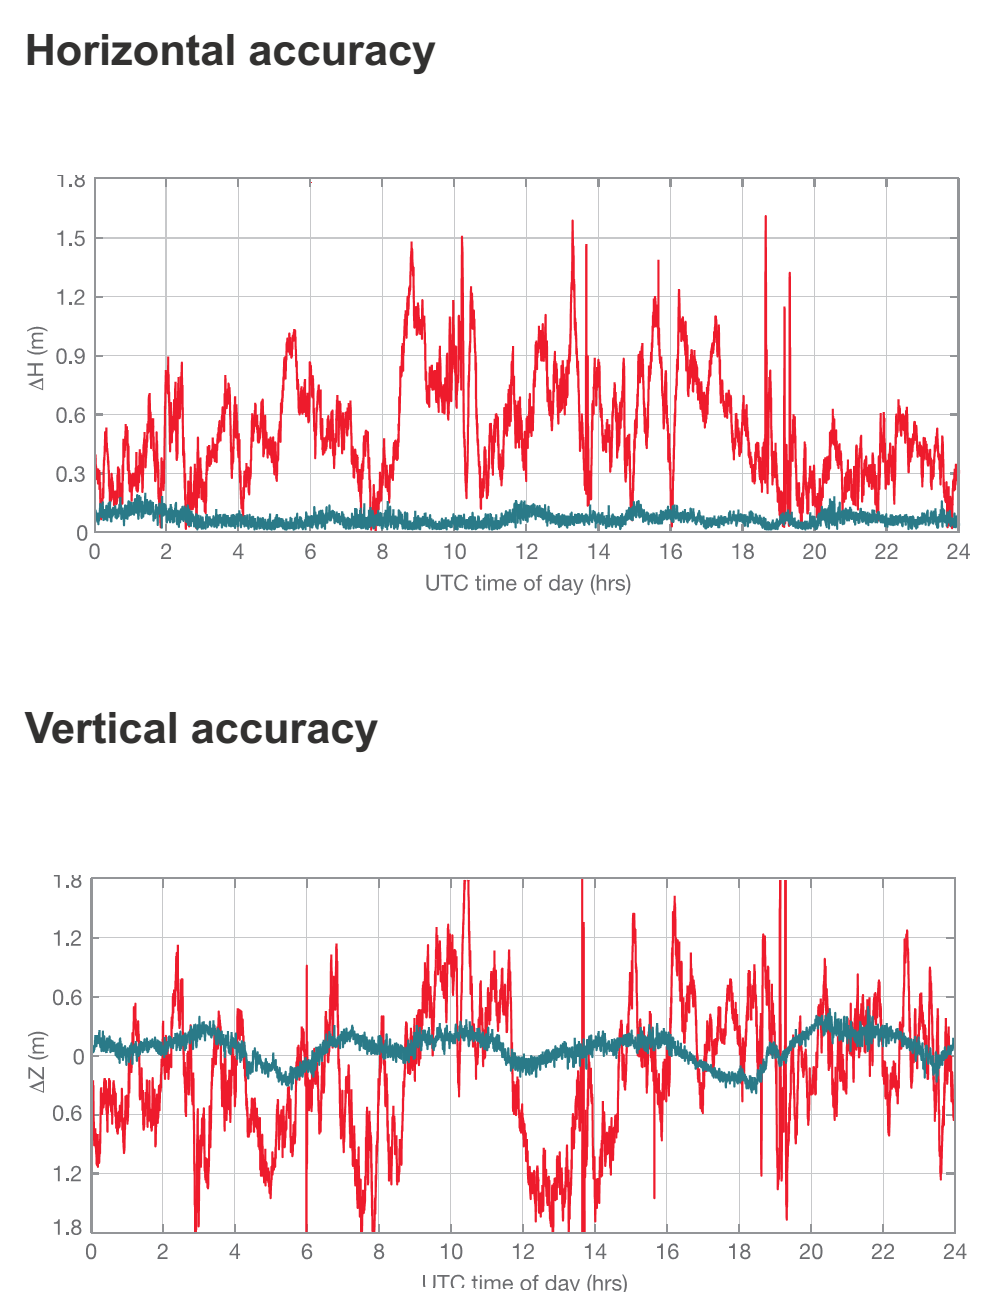
\includegraphics[height=.85\textheight]{pic/Ultra.png}
			\caption{Standard and Ultra solutions at a monitor site in Singapore.}
		\end{figure}
\end{frame}

%%%%%%%%%%%%%%%%%%%%%%%%%%%%%%%%%%%%%%%%%%%%%%%%%%%%%%%%%%%%%%%%%%%%%%%%
\section{Veripos demo}



%%%%%%%%%%%%%%%%%%%%%%%%%%%%%%%%%%%%%%%%%%%%%%%%%%%%%%%%%%%%%%%%%%%%%%%%
\section{Practical work}
\begin{frame}{NGB5}
	\begin{table}
		\centering
		\begin{minipage}[t]{\textwidth}%
			\resizebox{\columnwidth}{!}{%
				\begin{tabular}{lccccc} %{l|c|c|c|c}
					\toprule %\rowcolor{lightgray}
					Point & Frame & Lat $\phi$[deg]  & Long $\lambda$[deg]  & EllHt[m] & Notes\tabularnewline
					\midrule
					NGB5 & ETRF97 & 52 57 7.05304 & 01 11 1.44953 & 91.212 & at point\\
					NGB5 & ETRF97 & 52 57 7.05304 & 01 11 1.44953 & 91.392 & at ARP\\
					%\footnote{Antenna heigh = 0.18m.}
					NGB5 & ETRF97 & 52 57 7.05304 & 01 11 1.44953 & 91.434 & at antenna PCO\footnote{Antenna offset for ionsphere free solution is $2.545L_1-1.545L_2$ = $2.545*55.3-1.545*64.2=41.5mm$.}\\
					\textbf{NGB5} & ITRF2014 & \textbf{52 57 7.07209} & \textbf{01 11 1.42505} W & \textbf{91.488} & at antenna PCO\footnote{Converted from ETRF97 to ITRF2014 at epoch 2017-12-06.} \\
					\textbf{NGB5} & ITRF2014 & \textbf{5257.117868} & \textbf{0111.023751} W & \textbf{91.488} & at antenna PCO\footnote{To calculate error in meters at latitude $\phi$ of NGI, use $(\lambda_{NMEA}-\lambda_{truth})*1800$ and $(\phi_{NMEA}-\phi_{truth})*1200$. The 6th decimal place of GGA string is equivalent to 18mm N($\phi$) and 12mm E($\lambda$).
} \\		
					\bottomrule
				\end{tabular}%
			}
			\caption{Coordinates of NGB5}
		\end{minipage}
	\end{table}
\end{frame}
%in case of sec diference use 30 and 20m
% DDMM.123456


\begin{frame}{Veripos \$GPGGA NMEA strings}
	
	In Verpos provides two types of NMEA strings \$GPGGA and \$GPGST. \$GPGGA will behave differently in PPP mode with QA flag always 2 or 5. To obtain any information about solution we need to examine last flag before CRC(*).\\
	
	
	\begin{exampleblock}{Example}
		{\tiny{\$GPGGA,183324.00,5257.1178371,N,00111.0236798,W,\textbf{5},17,0.7,42.76,M,49.01,M,30.5,{\color{red}\textbf{0268}}*54}.}
	\end{exampleblock}
	
	Values for the flag indicate:	
	\begin{description}
		\item [0068]	ULTRA
		\item [0268]	$ULTRA^2$
		\item [0081]	APEX
		\item [0281]	$APEX^2$
		\item [1006]	$Standard^2$
	\end{description}
	%use  cut -d, -f15 *.txt | cut -d* -f1 | sort | uniq to extract data  
\end{frame}

\begin{frame}[plain]{Veripos \$GPGST NMEA strings}

	\begin{exampleblock}{Example}
		{\textit{\$GPGST,140545.00,3.81,0.02,0.01,81.00,0.02,0.01,0.02*57}.}
	\end{exampleblock}
	\vspace*{-1cm}
	\begin{table}
		\centering
		\begin{minipage}[t]{\textheight}%
			\resizebox{\columnwidth}{!}{%
				\begin{tabular}{lc} %{l|c|c|c|c}
					\toprule %\rowcolor{lightgray}
					Cell & Notes\tabularnewline
					\midrule
					0&Message ID \$GPGST\\
					1&UTC of position fix\footnote{Notice 18s offset to GPS time.}\\
					2&RMS value of the pseudorange or carrier phase (RTK/PPP) residuals\\
					3&Error ellipse semi-major axis 1 sigma error, in meters\\
					4&Error ellipse semi-minor axis 1 sigma error, in meters\\
					5&Error ellipse orientation, degrees from true north\\
					6&Latitude 1 sigma error, in meters\\
					7&Longitude 1 sigma error, in meters\\
					8&Height 1 sigma error, in meters\\
					9&The checksum data, always begins with *\\
					\bottomrule
				\end{tabular}%
			}
		\end{minipage}
	\end{table}
\end{frame}



%Final slide
% \setbeamercolor{background canvas}{bg=blueBgd!60}
% \plain{Questions?}



\end{document}
